\chapter{Diseño e implementación de un orquestador para tareas de tiempo real}

En los capítulos anteriores, se ha presentado el concepto de la Industria 4.0 y
los problemas que plantea, indicando que el paradigma del \textit{fog computing}
y las tecnologías de virtualización pueden ser una solución factible para
conseguir su implantación. Para apoyar este planteamiento, se ha decidido
implementar una herramienta de orquestación de tareas de tiempo real sobre
entornos distribuidos que sirva como prueba de concepto. En este capítulo, se
detalla el proceso seguido para su desarrollo, justificando las decisiones
de diseño tomadas y mostrando los de detalles más relevantes de la
implementación. Para terminar, se muestra una caracterización inicial del
rendimiento de la herramienta desarrollada.

\section{Objetivos y requisitos}

Como ya se ha explicado, la llegada de la Industria 4.0 supone un aumento muy
grande en la cantidad de datos generados en las plantas debido al IoT
industrial, datos que son necesarios para poder obtener gemelos digitales con un
nivel de detalle suficiente. Los nuevos sistemas ciber-físicos necesitan, por
tanto, procesar todos estos datos en tiempo real para poder tomar decisiones de
control en base a los mismos y garantizar una operación eficiente. Para ello, es
necesario poseer una capacidad de procesamiento elevada, mayor de la que
cualquier dispositivo individual pueda aportar. Aunque la computación en la nube
pueda parecer una solución natural a este problema, la enorme carga que pondría
sobre la red la constante transmisión de cantidades de datos tan grandes, así
como la latencia resultante de estas comunicaciones, hacen que no podamos
considerar esta plataforma como apropiada para dar cobijo a tareas con
restricciones temporales. En la sección \ref{sec:02-cloud_fog_edge}, se introduce
el paradigma \textit{fog} como una extensión de la nube más cercana a las
fuentes de datos. Según este modelo, los datos generados por los dispositivos
del borde de la red son procesados en nodos ubicados en la misma red local.
Aunque la potencia combinada de los dispositivos que conformen esta capa
\textit{fog} será menor que la que encontramos en la nube, puede ser suficiente
para las tareas de análisis de datos y toma de decisiones que se deben realizar
en las plantas, reduciendo así la presión sobre la red y garantizando unos
tiempos de respuesta muy inferiores.

Debido a esto, el modelo \textit{fog} se plantea como una posible plataforma
para la implementación de los nuevos sistemas ciber-físicos. Las tareas de
control industrial deben, entonces, distribuirse por los nodos de la capa
\textit{fog} de forma dinámica para dar respuesta a la carga de trabajo en todo
momento. Para que esta distribución de procesos sobre los nodos se produzca de
manera eficiente, es necesario hacer uso de las tecnologías de virtualización,
las cuales ya sirven para solucionar una problemática similar en la nube. Al
virtualizar los procesos, se abstraen las capas inferiores como son el hardware
o el sistema operativo, facilitando el despliegue de los mismos sobre
dispositivos con características dispares y unificando su desarrollo, dado que
no es necesario implementarlos para cada plataforma distinta). Así, se facilita
la escalabilidad de los procesos para dar respuesta a los cambios en la demanda.
En la sección \ref{sec:02-virtualization}, planteamos el uso de contenedores en vez
de máquinas virtuales para esto, apoyándonos en su carácter más liviano y su
mejor rendimiento para operaciones de entrada y salida.

Por tanto, en el modelo planteado es necesario desplegar las tareas de control
en forma de contenedores. Para explorar más este concepto, hemos decidido
implementar una herramienta que permita realizar esto sobre múltiples nodos. Los
objetivos de esta herramienta son:

\begin{table}[H]
    \centering
    \begin{tabular}{ |>{\columncolor[gray]{0.8}}l|p{0.7\textwidth}| }
        \hline
        Nombre      & Gestión de nodos                                       \\
        \hline
        Importancia & Alta                                                   \\
        \hline
        Descripción & Llevar un control de los dispositivos que conforman la
        capa \textit{fog} es una parte esencial de la implantación de este
        modelo.                                                              \\
        \hline
    \end{tabular}
    \caption{Objetivo 01 - Gestión de nodos.}
    \label{tab:04-obj01}
\end{table}

\begin{table}[H]
    \centering
    \begin{tabular}{ |>{\columncolor[gray]{0.8}}l|p{0.7\textwidth}| }
        \hline
        Nombre      & Gestión de tareas                                          \\
        \hline
        Importancia & Alta                                                       \\
        \hline
        Descripción & Las distintas tareas que se deben ejecutar sobre los nodos
        de la capa \textit{fog} deben estar recopiladas y centralizadas en el
        sistema.                                                                 \\
        \hline
    \end{tabular}
    \caption{Objetivo 02 - Gestión de tareas.}
    \label{tab:04-obj02}
\end{table}

\begin{table}[H]
    \centering
    \begin{tabular}{ |>{\columncolor[gray]{0.8}}l|p{0.7\textwidth}| }
        \hline
        Nombre      & Orquestación de tareas                                \\
        \hline
        Importancia & Muy alta                                              \\
        \hline
        Descripción & El sistema debe permitir a los usuarios desplegar las
        tareas definidas sobre los nodos de manera sencilla, controlando siempre
        que la ejecución de las tareas sobre cada nodo concreto sea viable. \\
        \hline
    \end{tabular}
    \caption{Objetivo 03 - Orquestación de tareas.}
    \label{tab:04-obj03}
\end{table}

\begin{table}[H]
    \centering
    \begin{tabular}{ |>{\columncolor[gray]{0.8}}l|p{0.7\textwidth}| }
        \hline
        Nombre      & Uso de software libre                                      \\
        \hline
        Importancia & Media                                                      \\
        \hline
        Descripción & Como parte de nuestro compromiso con el software libre, el
        sistema desarrollador deberá hacer uso siempre que sea posible de
        tecnologías abiertas.                                                    \\
        \hline
    \end{tabular}
    \caption{Objetivo 04 - Uso de software libre.}
    \label{tab:04-obj04}
\end{table}

A partir de estos objetivos, se han concretado una serie de requisitos que
deberá satisfacer la herramienta desarrollada.

\begin{table}[H]
    \centering
    \begin{tabular}{ |>{\columncolor[gray]{0.8}}l|p{0.5\textwidth}| }
        \hline
        Nombre                 & Añadir un nuevo nodo                       \\
        \hline
        Objetivos relacionados & \ref{tab:04-obj01}                         \\
        \hline
        Descripción            & Un usuario debe poder añadir al sistema un
        nuevo nodo que represente a un dispositivo de la capa \textit{fog}. Los
        datos proporcionados para el nuevo nodo deben permitir la conexión al
        mismo por SSH.                                                      \\
        \hline
    \end{tabular}
    \caption{Requisito 01 - Añadir un nuevo nodo.}
    \label{tab:04-req01}
\end{table}

\begin{table}[H]
    \centering
    \begin{tabular}{ |>{\columncolor[gray]{0.8}}l|p{0.5\textwidth}| }
        \hline
        Nombre                 & Obtener datos de los nodos                      \\
        \hline
        Objetivos relacionados & \ref{tab:04-obj01}                              \\
        \hline
        Descripción            & Un usuario debe poder obtener información sobre
        los nodos que hay registrados en el sistema, tanto de forma colectiva como
        detallada para un nodo concreto.                                         \\
        \hline
    \end{tabular}
    \caption{Requisito 02 - Obtener datos de los nodos.}
    \label{tab:04-req02}
\end{table}

\begin{table}[H]
    \centering
    \begin{tabular}{ |>{\columncolor[gray]{0.8}}l|p{0.5\textwidth}| }
        \hline
        Nombre                 & Modificar un nodo                               \\
        \hline
        Objetivos relacionados & \ref{tab:04-obj01}                              \\
        \hline
        Descripción            & Un usuario debe poder actualizar la información
        relativa a un nodo ya registrado en el sistema si fuera necesario.       \\
        \hline
    \end{tabular}
    \caption{Requisito 03 - Modificar un nodo.}
    \label{tab:04-req03}
\end{table}

\begin{table}[H]
    \centering
    \begin{tabular}{ |>{\columncolor[gray]{0.8}}l|p{0.5\textwidth}| }
        \hline
        Nombre                 & Eliminar un nodo                              \\
        \hline
        Objetivos relacionados & \ref{tab:04-obj01}                            \\
        \hline
        Descripción            & Un usuario debe poder eliminar del sistema un
        nodo cuando sea necesario.                                             \\
        \hline
    \end{tabular}
    \caption{Requisito 04 - Eliminar un nodo.}
    \label{tab:04-req04}
\end{table}

\begin{table}[H]
    \centering
    \begin{tabular}{ |>{\columncolor[gray]{0.8}}l|p{0.5\textwidth}| }
        \hline
        Nombre                 & Añadir una nueva tarea                         \\
        \hline
        Objetivos relacionados & \ref{tab:04-obj02}                             \\
        \hline
        Descripción            & Un usuario debe poder añadir al sistema tareas
        de tiempo real para su posterior despliegue sobre los nodos del mismo.
        Se deben aportar, por tanto, tanto los ficheros con la tarea como los
        atributos relativos a sus restricciones temporales.                     \\
        \hline
    \end{tabular}
    \caption{Requisito 05 - Añadir una nueva tarea.}
    \label{tab:04-req05}
\end{table}

\begin{table}[H]
    \centering
    \begin{tabular}{ |>{\columncolor[gray]{0.8}}l|p{0.5\textwidth}| }
        \hline
        Nombre                 & Obtener datos de las tareas              \\
        \hline
        Objetivos relacionados & \ref{tab:04-obj02}                       \\
        \hline
        Descripción            & Un usuario debe poder ver la información
        relativa a las tareas registradas en el sistema.                  \\
        \hline
    \end{tabular}
    \caption{Requisito 06 - Obtener datos de las tareas.}
    \label{tab:04-req06}
\end{table}


\begin{table}[H]
    \centering
    \begin{tabular}{ |>{\columncolor[gray]{0.8}}l|p{0.5\textwidth}| }
        \hline
        Nombre                 & Modificar una tarea                           \\
        \hline
        Objetivos relacionados & \ref{tab:04-obj02}                            \\
        \hline
        Descripción            & Un usuario debe poder actualizar una tarea ya
        presente en el sistema si fuera necesario.                             \\
        \hline
    \end{tabular}
    \caption{Requisito 07 - Modificar una tarea.}
    \label{tab:04-req07}
\end{table}

\begin{table}[H]
    \centering
    \begin{tabular}{ |>{\columncolor[gray]{0.8}}l|p{0.5\textwidth}| }
        \hline
        Nombre                 & Eliminar una tarea                           \\
        \hline
        Objetivos relacionados & \ref{tab:04-obj02}                           \\
        \hline
        Descripción            & Un usuario debe poder eliminar una tarea del
        sistema.                                                              \\
        \hline
    \end{tabular}
    \caption{Requisito 08 - Eliminar una tarea.}
    \label{tab:04-req08}
\end{table}

\begin{table}[H]
    \centering
    \begin{tabular}{ |>{\columncolor[gray]{0.8}}l|p{0.5\textwidth}| }
        \hline
        Nombre                 & Desplegar una tarea en un nodo            \\
        \hline
        Objetivos relacionados & \ref{tab:04-obj03}                        \\
        \hline
        Descripción            & Un usuario debe poder desplegar una tarea
        registrada en el sistema sobre un nodo también registrado.         \\
        \hline
    \end{tabular}
    \caption{Requisito 09 - Desplegar una tarea en un nodo.}
    \label{tab:04-req09}
\end{table}

\begin{table}[H]
    \centering
    \begin{tabular}{ |>{\columncolor[gray]{0.8}}l|p{0.5\textwidth}| }
        \hline
        Nombre                 & Eliminar una tarea de un nodo            \\
        \hline
        Objetivos relacionados & \ref{tab:04-obj03}                       \\
        \hline
        Descripción            & Un usuario debe poder eliminar una tarea
        previamente desplegada en un nodo cuando sea necesario.           \\
        \hline
    \end{tabular}
    \caption{Requisito 10 - Eliminar una tarea de un nodo.}
    \label{tab:04-req10}
\end{table}

\begin{table}[H]
    \centering
    \begin{tabular}{ |>{\columncolor[gray]{0.8}}l|p{0.5\textwidth}| }
        \hline
        Nombre                 & Garantizar la viabilidad de los conjuntos de tareas \\
        \hline
        Objetivos relacionados & \ref{tab:04-obj03}                                  \\
        \hline
        Descripción            & El sistema debe de garantizar en todo momento y
        en la medida de lo posible que las tareas que se ejecutan sobre un nodo
        dado son viables.                                                            \\
        \hline
    \end{tabular}
    \caption{Requisito 11 - Garantizar la viabilidad de los conjuntos de tareas.}
    \label{tab:04-req11}
\end{table}

\begin{table}[H]
    \centering
    \begin{tabular}{ |>{\columncolor[gray]{0.8}}l|p{0.5\textwidth}| }
        \hline
        Nombre                 & Despliegue usando contenedores                 \\
        \hline
        Objetivos relacionados & \ref{tab:04-obj03}                             \\
        \hline
        Descripción            & El despliegue de las tareas sobre los nodos se
        debe realizar mediante contenedores.                                    \\
        \hline
    \end{tabular}
    \caption{Requisito 12 - Despliegue usando contenedores.}
    \label{tab:04-req12}
\end{table}

\section{Diseño del sistema}
\label{sec:04-system_design}

A la hora de abordar el diseño de la herramienta, se nos planteaban varias
posibilidades. La solución más sencilla podría consistir de una aplicación
monolítica, de escritorio o web, que aglutinase toda la funcionalidad recogida
en los requisitos detallados en la sección anterior. Una aplicación monolítica
de este tipo, aunque no siempre es una mala opción, plantea varios problemas
como son su difícil escalabilidad o la complejidad creciente conforme se añaden
funcionalidades, lo que incrementa los costes de desarrollo y mantenimiento.
Además, el sistema que se desea crear se visualiza siendo usado por varios
usuarios. Se podría pensar, por ejemplo, en ingenieros de una fábrica que se
encargan del desarrollo y mantenimiento de sus sistemas de control, cada uno
usando su propio PC para llevar a cabo estas tareas a través de nuestra
herramienta. En una situación como esa, usar una aplicación monolítica es
inviable, dado que los usuarios deben trabajar de forma concurrente sobre un
conjunto de datos común.

La manera más sencilla para permitir esta colaboración y conseguir que todos los
usuarios trabajen sobre una misma base consiste en aplicar un modelo de
cliente-servidor. El sistema se modulariza, encapsulando la funcionalidad más
importante en un servidor y relegando las aplicaciones que usan los usuarios a
simples cascarones encargados de proporcionar una interfaz entre las
funcionalidades del sistema y ellos mismos. Una arquitectura de este tipo hace
más fácil controlar el acceso concurrente a los datos, evitando problemas de
integridad e incoherencia en los mismos. Además, debido a que los clientes no
tienen tantas responsabilidades, acaban siendo más simples y livianos, lo que
facilita su instalación en las máquinas de los usuarios. Es por todas estas
razones que se ha escogido la arquitectura cliente-servidor para el diseño del
sistema. En la figura \ref{fig:04-architecture} se puede ver un diagrama del
diseño propuesto para el sistema. Aquí se puede ver como el servidor contiene
toda la lógica relativa a los nodos, las tareas y el despliegue de éstas. Aunque
se podría haber planteado la separación de esta lógica en varios microservicios,
esta opción se descartó debido a que no se espera que el sistema tenga que ser
usado por muchos usuarios a la vez ni su carga pueda elevarse de forma
considerable, por lo que los beneficios de escalabilidad que este tipo de diseño
podría aportar son innecesarios y se ven enormemente contrarrestados por la
complejidad que añaden.

\begin{figure}
    \centering
    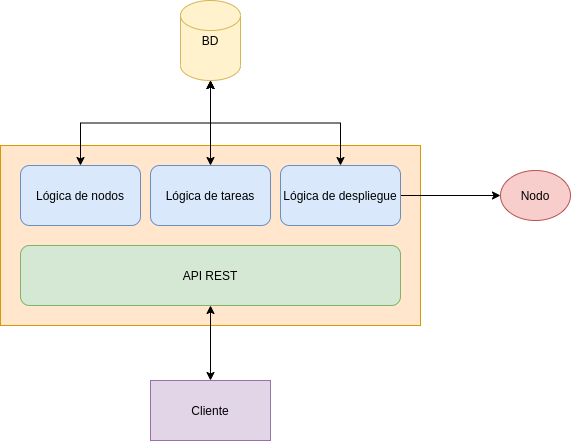
\includegraphics[width=0.8\textwidth]{04-implementation/architecture.png}
    \caption{Diagrama de arquitectura del sistema.}
    \label{fig:04-architecture}
\end{figure}

Volviendo a la figura \ref{fig:04-architecture}, apreciamos que el servidor
también controla el acceso a la base de datos donde se almacena toda la
información sobre los nodos y las tareas. Para esta base de datos, como ya se
indicó en la sección \ref{sec:01-tools}, se ha decidido MongoDB, que es un gestor
de bases de datos documentales y no estructuradas. También se puede comprobar en
el diagrama que el servidor expone todas las funcionalidades del sistema a
través de una API (\textit{Application Programming Interface}). Esta API sigue
el patrón arquitectónico REST (\textit{REpresentation State Transfer}), el cuál
fue introducido en el año 2000 por Roy Fielding en su tesis doctoral
\cite{fielding_architectural_2000}. Simplificando los conceptos que se
desarrollan en esta tesis, podemos identificar las siguientes características
fundamentales del patrón REST:

\begin{itemize}
    \item La interfaz se diseña en torno a recursos, los cuáles son conjuntos de
          información.
    \item Cada recurso está identificado de forma única mediante una URI.
    \item Las operaciones se realizan mediante peticiones HTTP hacia la URI del
          recurso objetivo.
    \item La operación a realizar viene definida por el verbo HTTP usado en la
          petición (\texttt{GET}, \texttt{POST}, \texttt{PUT}, \texttt{PATCH} o
          \texttt{DELETE}).
    \item El servidor no almacena estado alguno, de forma que cada petición debe
          contener toda la información necesaria como para poder darle respuesta.
    \item Para la transferencia de información, se utilizan formatos bien
          definidos como JSON o XML.
\end{itemize}

La aplicación del patrón REST al diseño de interfaces hace que sea más sencillo
estructurar el acceso a la información que contiene un servicio concreto, además
de simplificar también el flujo de trabajo entre cliente y servidor. Para
aplicar REST al diseño de un servicio concreto, se debe identificar cuáles son
los recursos con los que trabaja y qué operaciones permite sobre los mismos. En
el caso de nuestro sistema, tenemos los recursos detallados en las tablas
\ref{tab:04-node_resource} y \ref{tab:04-task_resource}, mientras que las
operaciones posibles se presentan en la sección \ref{sec:server-design}.

\begin{table}[H]
    \centering
    \begin{tabular}{ |>{\columncolor[gray]{0.8}}l|p{0.8\textwidth}| }
        \hline
        Recurso   & Nodo           \\
        \hline
        Atributos &
        \begin{itemize}
            \item ID
            \item Nombre
            \item Dirección IP
            \item Usuario (utilizado para la conexión SSH)
            \item CPU (modelo del procesador)
            \item Arquitectura de CPU (p. ej., \texttt{ARMv7})
            \item Número de núcleos de la CPU
            \item Frecuencia de reloj
            \item RAM
            \item Dispositivos (p. ej., \texttt{/dev/null})
            \item Tareas (que se están ejecutando en el nodo)
        \end{itemize} \\
        \hline
    \end{tabular}
    \caption{Definición del recurso nodo.}
    \label{tab:04-node_resource}
\end{table}

\begin{table}[H]
    \centering
    \begin{tabular}{ |>{\columncolor[gray]{0.8}}l|p{0.8\textwidth}| }
        \hline
        Recurso   & Tarea          \\
        \hline
        Atributos &
        \begin{itemize}
            \item ID
            \item Nombre
            \item Tiempo de ejecución (\textit{runtime})
            \item Límite de tiempo (\textit{deadline})
            \item Período (\textit{period})
            \item Dispositivos (a los que necesita acceder)
            \item Capacidades (p. ej., \texttt{SYS\_NICE})
            \item ID del desplegable (fichero tar con código fuente y \texttt{Dockerfile})
        \end{itemize} \\
        \hline
    \end{tabular}
    \caption{Definición del recurso tarea.}
    \label{tab:04-task_resource}
\end{table}

Como ya se ha indicado, aplicar una arquitectura cliente-servidor como esta
permite reducir al máximo la lógica que contienen los clientes, los cuáles solo
tienen que ocuparse de mostrar la interfaz, comprobar las entradas de los
usuarios y realizar la comunicación con el servidor. Además, el hecho de que el
servidor exponga una API estandarizada facilita enormemente la implementación de
múltiples tipos de aplicaciones cliente, incluso para distintas plataformas (p.
ej., móvil, web o escritorio). Estos clientes sencillamente tienen que consumir
recursos de la interfaz y pueden ofrecer a sus usuarios exactamente las mismas
funcionalidades que los demás. Esta separación de responsabilidades facilita
también el desarrollo y mantenimiento del software, ya que se trata de partes
completamente independientes y separadas que solo deben atenerse a la
especificación de la interfaz mediante la que se conectan.

Por último, también se ha decidido en esta fase de diseño implementar una imagen
Docker, que es el motor de contenedores usado por el sistema, para facilitar el
despliegue de tareas de tiempo real usando el sistema planteado. El
funcionamiento de esta imagen, así como los detalles de diseño e implementación
de las demás partes del sistema, se explican de forma extensiva en las
siguientes secciones de este capítulo. Todo el código desarrollado del que se va
a hablar se encuentra disponible en los repositorios de GitHub del
proyecto\footnote{Repositorio del servidor:
    \url{https://github.com/Varrrro/shipyard-server}}\footnote{Repositorio del
    cliente: \url{https://github.com/Varrrro/shipyard-cli}}\footnote{Repositorio de
    la librería: \url{https://github.com/Varrrro/libshipyard}}.

\section{Servidor maestro}

Tal y como se ha descrito en la sección anterior, el servidor es la parte del
sistema desarrollado que encapsula la lógica principal encargada de llevar a
cabo las funcionalidades deseadas. En esta sección se ahonda en las decisiones
de diseño tomadas para este componente, además de mostrar algunas partes
interesantes de la implementación y las técnicas de prueba e integración
continua aplicadas.

\subsection{Diseño e implementación}
\label{sec:server-design}

A la hora de estructurar el servidor, decidimos hacer una separación por
dominios, de forma que tenemos por un lado la lógica relativa a las
funcionalidades de los nodos y, por otro, la de las tareas. A su vez, también
realizamos una división de responsabilidades, diferenciando entre controladores
y servicios.

Los controladores definen las rutas y operaciones posibles en la API REST del
servidor. Este servidor recibe peticiones HTTP para las rutas que expone, las
cuáles se manejan con distintos controladores dependiendo del verbo HTTP usado.
Estos controladores se encargan entonces de validar los datos recibidos en la
petición, gestionar la autenticación y construir las respuestas con el código de
estado adecuado, llamando a funciones de los servicios para realizar las
operaciones. En los servicios se implementa la lógica encargada de llevar a cabo
estas operaciones como tal, conectando con la base de datos para la gestión de
nodos y tareas, además de llevar a cabo el despliegue de éstas. Como ya se ha
indicado, la lógica se divide también por dominio, de forma que tenemos unos
controladores para las operaciones sobre los nodos y otros separados para las
que ocurren sobre las tareas. Lo mismo ocurre con la lógica de estas operaciones
en los servicios. Para las acciones de orquestación de tareas, además, los
servicios hacen uso de un paquete independiente que implementa estas
funcionalidades concretas. El diagrama de la figura
\ref{fig:04-server_architecture} refleja esta arquitectura que se acaba de
describir.

En cuanto a las operaciones concretas que se pueden realizar mediante la API
REST del servidor, se han definido e implementado las siguientes:

\begin{figure}
    \centering
    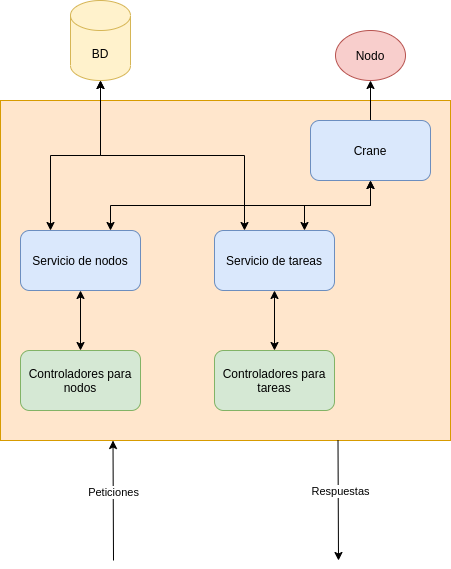
\includegraphics[width=0.9\textwidth]{04-implementation/server.png}
    \caption{Diagrama de arquitectura del servidor.}
    \label{fig:04-server_architecture}
\end{figure}

\begin{itemize}
    \item \texttt{GET /nodes}

          Con esta operación, se obtiene una lista completa de los nodos
          presentes en el sistema. En caso de ocurrir algún error (p. ej., en la
          conexión con la base de datos), el servidor devuelve un una respuesta
          500 (\textit{Internal Server Error}). Si no hay ningún problema, la
          respuesta tiene el código de estado 200 (\textit{Ok}) y contiene en su
          cuerpo la lista de nodos. Cabe destacar que en esta lista de nodos no
          se muestra toda la información presente en la base de datos sobre los
          mismos, sino que se ocultan algunos datos como son el usuario SSH, los
          dispositivos que tiene o los detalles de la CPU.

    \item \texttt{POST /nodes}

          Esta operación permite crear un nuevo nodo, debiendo incluir en el
          cuerpo de la petición los datos del nuevo nodo. No es necesario
          proporcionar valores para todos los atributos definidos en la tabla
          \ref{tab:04-node_resource}, sino que solo son requeridos el nombre,
          dirección IP y número de núcleos de la CPU del nuevo nodo. El nombre
          dado debe ser único, devolviendo el servidor una respuesta 409
          (\textit{Conflict}) si ya está en uso por otro nodo del sistema.

          La petición HTTP que recibe el servidor debe contener en la cabecera
          \textit{Authorization} unas credenciales de autenticación de tipo
          básico, es decir, usuario y contraseña codificados con Base64. Este
          usuario y contraseña son los usados por el servidor para establecer la
          conexión SSH inicial con el nodo. Esta conexión inicial sirve para
          añadir los datos del nodo al fichero \texttt{known\_hosts} del
          servidor con el que se regulan las conexiones SSH conocidas y copiar
          la clave pública de éste al fichero \texttt{authorized\_keys} del
          nodo. Esto permite que las siguientes conexiones SSH que deba realizar
          el servidor usen esta clave para la autenticación, de forma que no sea
          necesario usar la contraseña y aumentando la seguridad.

          Si los datos enviados en el cuerpo de la petición no son correctos, el
          controlador devuelve una respuesta 400 (\textit{Bad Request}). En caso
          de no poder crear el nodo por cualquier otro motivo, se devuelve un
          código 500. La ejecución correcta de esta operación produce una
          respuesta con código de estado 200 y con el nuevo recurso recién
          creado en el cuerpo.

    \item \texttt{GET /nodes?name=<node\_name>}

          Como se puede suponer por el verbo HTTP y la ruta usadas, esta
          operación permite obtener la información detallada de un nodo
          concreto, el cuál se identifica por el nombre proporcionado. Esta
          operación y \texttt{GET /nodes} comparten controlador, comprobándose
          al inicio de éste si en la URI de la petición se encuentra el
          parámetro de consulta \textit{name} para decidir si se llama a la
          función del servicio de nodos que devuelve la lista o a la que
          devuelve los detalles de uno concreto. A diferencia de lo que ocurría
          con esta otra operación, en este caso sí que se devuelven todos los
          atributos del nodo indicado junto con la respuesta 200. Si no se
          encuentra en la base de datos ningún nodo con el nombre indicado, la
          respuesta devuelta tiene un código de estado 404 (\textit{Not Found}).

    \item \texttt{GET /nodes/<node\_id>}

          Esta operación es idéntica a la anterior, siendo la única diferencia
          que la identificación del nodo cuyos detalles se desean obtener se
          realiza por su ID. Esta operación también devuelve una respuesta 200
          con los datos del nodo en el cuerpo en caso de encontrarse en la base
          de datos y un código 404 en caso contrario. También puede devolver una
          raspuesta 409 si el ID dado no es válido, es decir, si no cumple con
          el formato de ID de MongoDB.

    \item \texttt{PUT /nodes/<node\_id>}

          Con esta operación se pueden modificar los atributos de un nodo ya
          existente en el sistema. En el cuerpo de la petición se incluyen solo
          los atributos cuyo valor se desea cambiar junto con estos nuevos
          valores. Si el formato del cuerpo de la petición no es correcto, el
          controlador de la ruta devuelve una respuesta 409. También se devuelve
          este código si el ID indicado no es válido. Si no se encuentra en la
          base de datos del sistema ningún nodo con el ID dado, se devuelve una
          respuesta 404. En caso de realizarse correctamente la operación, la
          respuesta tiene el código de estado 200 y contiene en su cuerpo todos
          los datos del recurso actualizado. Cabe destacar que, si alguno de los
          atributos modificados es el nombre, la IP, el usuario SSH o la lista
          de dispositivos del nodo, el servidor procede a eliminar del mismo
          todas las tareas que tuviera ejecutándose con el fin de evitar
          inconsistencias y estados no recuperables en el sistema. En el
          diagrama de la figura \ref{fig:04-update_node} se refleja este
          comportamiento, además del resto de acciones que lleva a cabo el
          servidor para realizar esta operación.

          \begin{figure}
              \centering
              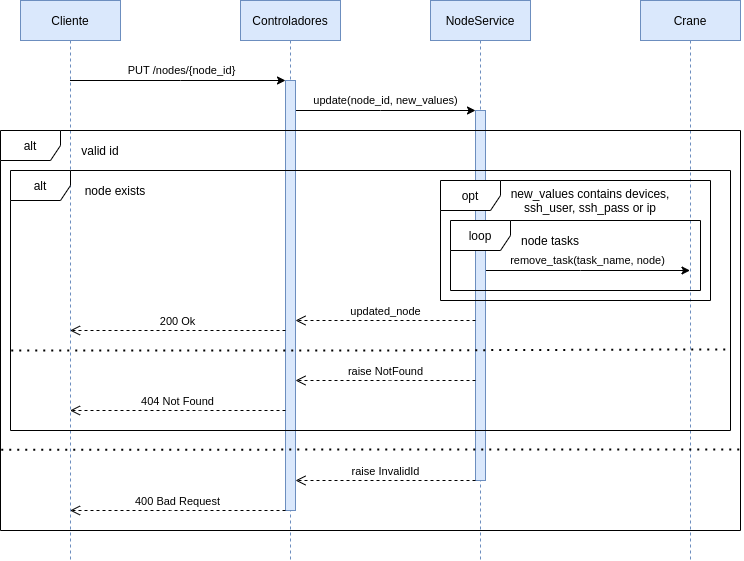
\includegraphics[width=\textwidth]{04-implementation/update-node.png}
              \caption{Diagrama de secuencias de la operación de actualización de un nodo.}
              \label{fig:04-update_node}
          \end{figure}

    \item \texttt{DELETE /nodes/<node\_id>}

          Esta operación permite eliminar un nodo del sistema. Las peticiones no
          necesitan contener ningún dato en el cuerpo, siendo solo necesario
          indicar en la propia ruta de la petición el ID del nodo a eliminar. Si
          este ID no es válido, el controlador devuelve una respuesta 409,
          mientras que si no se encuentra ningún nodo con este ID la respuesta
          es 404. Si la eliminación del recurso se realiza correctamente, la
          respuesta tiene el código de estado 200 y contiene en su cuerpo los
          datos del recurso recién eliminado. Al igual que ocurría con la
          modificación, el sistema se asegura de parar todas las tareas que se
          estuvieran ejecutando sobre el nodo que se elimina y borrarlas del
          mismo, de forma que no queden «restos» en el dispostivo.

    \item \texttt{GET /tasks}

          De forma análoga a la operación \texttt{GET /nodes}, ésta devuelve la
          lista de tareas que están almacenadas en la base de datos del sistema.
          El cuerpo de la respuesta contiene esta lista con el código de estado
          200 si la operación se ha podido realizar correctamente, devolviendo
          el código 500 en caso contrario.

    \item \texttt{POST /tasks}

          Permite añadir una nueva tarea al sistema. A diferencia de las demás
          operaciones, la cabecera \textit{content-type} de las peticiones para
          esta operación, que es la que regula el tipo de contenido, no tiene el
          valor \texttt{application/json}, sino que se usa
          \texttt{multipart/form-data}. Este tipo de contenido se compone de
          múltiples campos, los cuáles pueden ser textuales o archivos, lo cuál
          es necesario para esta operación dado que es necesario aportar tanto
          los metadatos de la tarea en formato JSON como un fichero
          \texttt{tar.gz} con el código fuente y la definición de la imagen
          Docker. El controlador de esta operación se encarga de extraer todos
          estos datos de los dos campos del cuerpo de la petición y, entonces,
          llamar a la función del servicio encargada de realizar la inserción de
          la tarea en la base de datos, devolviendo el controlador una respuesta
          200 si la operación se realiza correctamente. Si el formato de la
          petición recibida es incorrecto (p. ej., falta alguno de los campos),
          se devuelve una respuesta 400. Además, el nombre de la nueva tarea
          debe ser único, obteniendo una respuesta 409 en caso de no serlo. Si
          no se puede crear la tarea por cualquier otra razón, la respuesta
          obtenida es 500.

    \item \texttt{GET /tasks?name=<task\_name>}

          Con esta operación se pueden obtener los detalles de una tarea
          concreta, la cuál se identifica a partir del nombre indicado en el
          parámetro de consulta \textit{name} de la petición. Al igual que
          ocurría con la operación \texttt{GET /nodes?name=<node\_name>}, el
          controlador que da respuesta a esta operación es compartido con el de
          \texttt{GET /tasks}. Al inicio de la ejecución, el controlador
          comprueba la presencia del parámetro \textit{name} en la petición,
          devolviendo los detalles de la tarea o la lista completa de tareas
          según si está presente o no. En caso de operación correcta, la
          respuesta 200 incluye en el cuerpo los datos del recurso deseado a
          excepción del fichero \texttt{tar.gz} con su código fuente. Si este
          recurso no se encuentra, el código devuelto es 404, devolviendo 500 en
          cualquier otro caso.

    \item \texttt{GET /tasks/<task\_id>}

          Al igual que la operación anterior, ésta también devuelve los detalles
          de una tarea, aunque en este caso se usa el ID de la misma para su
          identificación. Si este ID no es válido, el controlador devuelve una
          respuesta 400; mientras que si no se encuentra en la base de datos
          ninguna tarea con este ID, la respuesta es 404. Esta operación tampoco
          devuelve el fichero de despliegue asociado a la tarea. Si no se puede
          realizar la operación, el controlador devuelve una respuesta 500.

    \item \texttt{PUT /tasks/<task\_id>}

          Modificación de una tarea. Como ocurría en la operación de creación de
          tareas, las peticiones también tienen el tipo de contenido
          \texttt{multipart/form-data}. Como diferencia, no es necesario que la
          petición contenga tanto el dichero \texttt{tar.gz} con el código
          fuente como el JSON con los atributos, sino que solo debe contener lo
          que se vaya a actualizar. Antes de modificar la tarea, el servidor se
          asegura de eliminarla de cualquier nodo en el que se estuviera
          ejecutando para evitar inconsistencias en el sistema. Si el ID dado o
          el formato del cuerpo de la petición no son válidos, el controlador
          devuelve una respuesta 400. Si no se encuentra en la base de datos
          ninguna tarea con el ID indicado, se devuelve un 404. En caso de
          realizarse la operación correctamente, la respuesta devuelta tiene el
          código 200 y contiene en su cuerpo el recurso actualizado. Si no se
          puede realizar la operación por cualquier otra razón, devuelve una
          respuesta 500.

    \item \texttt{DELETE /tasks/<task\_id>}

          Elimina una tarea de la base de datos del sistema, identificada por el
          ID indicado en la propia petición. Si no se encuentra ninguna tarea
          con dicho ID, devuelve 404. Si este ID no es válido, devuelve 400. Si
          no se puede realizar la operación por cualquier otra razón, devuelve
          500. Cuando la eliminación se completa de forma satisfactoria, el
          controlador devuelve una respuesta con código 200 y con el recurso
          recién eliminado en el cuerpo.

    \item \texttt{POST /nodes/<node\_id>/tasks?task\_id=<task\_id>}

          Esta operación permite el despliegue de una tarea dada en un nodo. Es,
          quizás, la operación más compleja que realiza el servidor. Se recibe
          una petición en cuya ruta se se encuentra el ID del nodo, aportándose
          el de la tarea como un parámetro de consulta (\textit{query}). Si este
          parámetro de consulta no está presente en la petición, el controlador
          devuelve inmediatamente una respuesta 400. Si todos los valores están
          presentes, se llama entonces a la función del servicio encargada de
          llevar a cabo el despliegue.

          Esta función convierte los IDs a los propios de MongoDB, lanzando un
          error \texttt{InvalidId} en caso de que su formato no sea correcto. El
          controlador devolvería entonces una respuesta 400 al cliente. El
          servicio puede devolver un error \texttt{NotFound} si no encuentra en
          la base de datos los recursos deseados, error que captura el
          controlador para generar una respuesta 404. Si los IDs se corresponden
          con recursos existentes en el sistema, el servicio procede a comprobar
          que el nodo posea todos los dispositivos que necesita la tarea. Si no
          es así, el servicio lanza un error \texttt{MissingDevices} que es
          capturado por el controlador, que genera una respuesta 500. La última
          comprobación que se realiza es la de la viabilidad de la ejecución del
          conjunto de tareas que se obtendría al añadir la nueva tarea a las que
          ya se están ejecutando en el nodo. Tanto para realizar esta
          comprobación como para llevar a cabo el despliegue como tal, el
          servicio se apoya en el paquete interno \textit{crane} que ya fue
          introducido al inicio de esta sección. La función
          \texttt{check\_feasibility} de este paquete es comprueba esta
          viabilidad. Esta función recibe el conjunto de tareas y el número de
          núcleos de la CPU del nodo objetivo. Con estos datos, se calcula la
          utilización de CPU para determinar si la ejecución es viable o no
          \cite{zhang_schedulability_2009}. Cabe destacar que, si el nodo tiene
          más de un núcleo (multiprocesador), esta comprobación de la
          utilización no es condición suficiente para asegurar la viabilidad del
          conjunto de tareas, aunque en esta primera versión de la herramienta
          no se gestiona esta situación.

          \begin{figure}
              \centering
              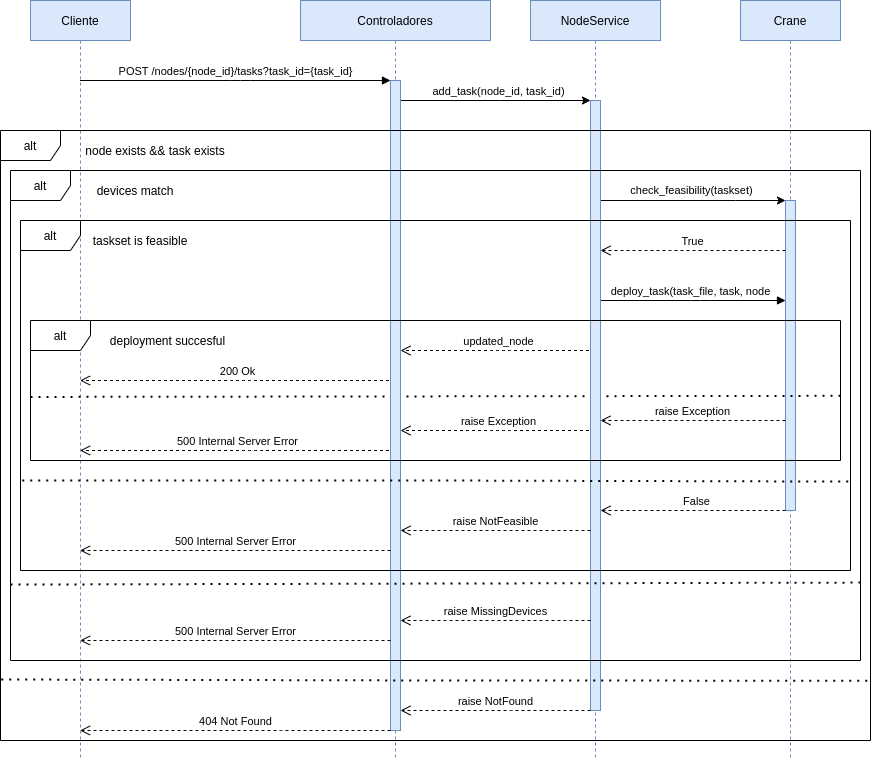
\includegraphics[width=\textwidth]{04-implementation/deploy-task.png}
              \caption{Diagrama de secuencias de la operación de despliegue de una tarea.}
              \label{fig:04-deploy_task}
          \end{figure}

          Si la función \texttt{check\_feasibility} determina que el conjunto de
          tareas es viable, entonces se ejecuta otra función del paquete
          \textit{crane} para realizar el despliegue: \texttt{deploy\_task}.
          Esta función recibe como entrada el fichero \texttt{tar.gz} de la
          tarea, así como sus metadatos y los del nodo. Con estos datos, se
          establece una conexión con el demonio Docker del nodo mediante SSH,
          obteniendo un cliente con el que se construye la imagen a partir del
          fichero \texttt{tar.gz} y se lanza el contenedor. Los parámetros de
          planificación de la tarea (tiempo de ejecución, límite de tiempo y
          período) se le pasan al contenedor como variables de entorno, las
          cuáles luego usará la librería para fijar la planificación.

          Cualquier tipo de excepción que se lance durante este despliegue será
          capturada por el controlador para generar una respuesta 500. Si la
          operación se realiza correctamente, el servidor responde con una
          respuesta 200 que contiene en su cuerpo los detalles del nodo
          actualizado, incluyendo ya en su lista de tareas la que se acaba de
          añadir. Todo este proceso que se acaba de describir para realizar la
          operación de despliegue se puede observar de manera esquematizada en
          el diagrama de secuencias de la figura \ref{fig:04-deploy_task}.

    \item \texttt{DELETE /nodes/<node\_id>/tasks/<task\_id>}

          Esta operación permite parar la ejecución de una tarea desplegada en
          un nodo concreto, elmininándola del mismo. Las peticiones recibidas
          para esta operación contienen en la ruta los valores de los IDs del
          nodo y la tarea en cuestión. El controlador entonces llama a la
          función del servicio encargada de realizar la operación.

          Lo primero que hace el servicio es comprobar si están presentes en la
          base de datos algunos recursos con los IDs proporcionados, lanzando un
          error \texttt{NotFound} en caso de no encontrarlos. Este error es
          entonces capturado por el controlador, que genera una respuesta 404
          para el cliente. Si al buscar los recursos en la base de datos resulta
          que los IDs no son válidos, se lanza un error \texttt{InvalidId}, para
          el que el controlador crea una respuesta 400.

          Si los recursos existen, el servicio entonces ejecuta la función
          \texttt{remove\_task} del paquete \textit{crane} para que se lleve a
          cabo la eliminación. Al igual que ocurría en la de despliegue de
          tareas, se crea un cliente para el servidor Docker del nodo mediante
          SSH usando las claves almacenadas. A través de este cliente, se
          elimina el contenedor en el que se ejecuta la tarea y, también, la
          imagen asociada. Una vez termina esta operación, se actualiza la base
          de datos para quitar la tarea de la lista que tiene asociada el nodo.
          Si durante la eliminación ocurre algún error, el controlador la
          captura y devuelve una respuesta 500 al cliente. Si la operación se
          realiza correctamente, la respuesta tiene un código de estado 200 y
          contiene en su cuerpo los datos actualizados del nodo, ya sin la tarea
          en su lista de tareas.
\end{itemize}

Gracias al uso de la librería \textit{hug}, la implementación de los
controladores es extremadamente sencilla. Cada controlador es una simple función
Python que, mediante decoradores, se enlaza con una operación concreta del
servidor a la que da respuesta. En el listado \ref{lst:04-post_node_tasks}, se
presenta el controlador de la operación de despligue de tareas. Como se puede
observar, es con el decorador \lstinline{@hug.post} con el que indicamos que se
debe ejecutar esta función cuando se reciba una petición POST para la ruta
\texttt{/nodes/<node\_id/tasks}\footnote{La ruta \texttt{/nodes} es la base para
    todos los controladores de los nodos, por eso no se muestra en el decorador.}.
Se definen aquí también las variables de ruta presentes, que en este caso es el
ID del nodo.

\begin{lstlisting}[
    language=Python,
    caption={Controlador de la operación de despliegue de tareas.},
    label={lst:04-post_node_tasks},
    showstringspaces=false
]
@hug.post('/{node_id}/tasks')
def post_node_tasks(node_id: str, response, task_id: str = None):
    if task_id is None:
        response.status = hug.HTTP_BAD_REQUEST
        return {
            'error': 'No task ID was specified in the request'
        }

    try:
        result = NodeService.add_task(node_id, task_id)
        if result is None:
            response.status = hug.HTTP_INTERNAL_SERVER_ERROR
            return {'error': 'Unable to add task to node.'}
        return Node.Schema().dump(result)
    except InvalidId as e:
        response.status = hug.HTTP_BAD_REQUEST
        return {'error': str(e)}
    except NotFound as e:
        response.status = hug.HTTP_NOT_FOUND
        return {'error': str(e)}
    except (NotFeasible, MissingDevices) as e:
        response.status = hug.HTTP_INTERNAL_SERVER_ERROR
        return {'error': str(e)}
    except Exception:
        response.status = hug.HTTP_INTERNAL_SERVER_ERROR
        return {'error': 'Unable to add task to node.'}   
\end{lstlisting}

Las funciones definidas como controladores con \textit{hug} reciben
estas variables de ruta como argumentos, teniendo también los posibles
parámetros de consulta (\texttt{task\_id}) y los objetos propios de la
comunicación HTTP (p. ej., \texttt{request}, \texttt{response}, \texttt{body}).
Observando el listado, se aprecia claramente cómo los controladores se encargan
solo de comprobar que el formato de la petición sea el correcto, llamar a la
función del servicio apropiada para realizar la operación y construir la
respuesta que corresponda en base al resultado de la misma, tal y como se
describía anteriormente.

\begin{lstlisting}[
    language=Python,
    caption={Función del servicio de tareas para la creación de tareas.},
    label={lst:04-task_service_create},
    showstringspaces=false
]
@staticmethod
def create(
    new_task: Task,
    file_name: str,
    file_body: BytesIO
    ) -> str:

    result = db.tasks.find_one({'name': new_task.name})
    if result is not None:
        raise AlreadyPresent(
            'A task already exists with the given name.'
        )

    file_id = fs.put(file_body, filename=file_name)
    new_task.file_id = file_id

    new_id = db.tasks.insert_one(Task.Schema(
        exclude=['_id']).dump(new_task)).inserted_id
    return str(new_id)
\end{lstlisting}

Por otro lado, en el listado \ref{lst:04-task_service_create} se muestra la
función del servicio de tareas que implementa la lógica encargada de la creación
de éstas. El objeto \texttt{db}, como se puede suponer, es la conexión con la
base de datos que mantiene el servidor. Esta función concreta tiene una
particularidad con respecto a las demás: se debe almacenar también el fichero
\texttt{tar.gz} con el código fuente y la definición de imagen de la tarea. Para
ello, usamos GridFS, que es la especificación de MongoDB para el almacenamiento
de ficheros de gran tamaño. De esta forma, se pueden almacenar los ficheros en
colecciones normales de MongoDB sin necesitar de otro tipo de almacenamiento. Al
igual que el objeto \texttt{db} era la conexión con la base de datos MongoDB,
\texttt{fs} es la conexión con la parte de GridFS. Entonces, para añadir una
nueva tarea al sistema, primero se añade el fichero con \texttt{fs.put()} y, con
el ID recién obtenido para el mismo, se crea el nuevo documento en la colección
de tareas.

Otro aspecto a destacar es el uso de \texttt{BytesIO} para el acceso al fichero.
Cuando el controlador de la operación \texttt{POST /tasks} recibe una nueva
petición, extrae el contenido del fichero del cuerpo de la misma y lo escribe a
un objeto de este tipo. A todos los efectos, un objeto \texttt{BytesIO} actúa
como un archivo normal, con la diferencia de que sus datos se almacenan
directamente en memoria en vez de en el sistema de archivos. Al usar este
mecanismo, conseguimos hacer que el proceso de inserción de la tarea sea más
rápido, dado que no tenemos que acceder a disco duro ni tenemos que trabajar con
ficheros.

Como se ha indicado en la sección \ref{sec:04-system_design}, la API REST usa el
formato estándar de codificación de datos JSON para la transmisión de
información entre el servidor y los clientes. La mayoría de las peticiones y
respuetas contienen en sus cuerpos una representación de los recursos del
sistema en este formato. Para que la serialización de los objetos Python a JSON
y viceversa se realice de forma más sencilla, se ha usado la librería
\textit{marshmallow}. Esta librería nos permite definir esquemas de datos para
los recursos del sistema que, además de ayudar con la serialización y
deserialización, proporciona un mecanismo de validación automática sobre los
datos recibidos de los clientes.

\subsection{Prueba}

Para asegurar el correcto funcionamiento del código implementado, se han escrito
pruebas unitarias. Este tipo de pruebas se centran en validar el comportamiento
de partes individuales del sistema, aíslandolas del resto. En nuestro caso, las
pruebas se realizan para las funciones de los controladores y los servicios. La
librería \textit{unittest}, que forma parte de la librería estándar de Python,
proporciona los mecanismos que se han utilizado para implementar estas pruebas.
Con esta librería, se definen clases \texttt{TestCase}, que son las unidades
individuales de prueba para un componente concreto. Las funciones de estas
clases son las que comprueban que las salidas obtenidas para determinadas
entradas son las correctas en las funciones individuales del componente dado.
Para nuestro servidor, se han definido cuatro clases \texttt{TestCase} para los
cuatro componentes principales: controladores de los nodos, controladores de las
tareas, servicio de nodos y servicio de tareas.

\begin{lstlisting}[
    language=Python,
    caption={Prueba unitaria del controlador para el despliegue de tareas.},
    label={lst:04-post_node_tasks_test}
]
def test_post_node_tasks(self):
    response = hug.test.call(
        'POST', controllers, f'{test_nodes[0]._id}/tasks',
        params={
            'task_id': 'Test'
    })
    self.assertEqual(response.status, hug.HTTP_OK)
    self.assertIsNotNone(response.data)

    response = hug.test.call(
        'POST', controllers, f'{ObjectId()}/tasks', params={
            'task_id': 'Test'
    })
    self.assertEqual(response.status, hug.HTTP_NOT_FOUND)
    self.assertIsNotNone(response.data)
    self.assertIsInstance(response.data['error'], str)

    response = hug.test.call(
        'POST', controllers, f'{test_nodes[0]._id}/tasks')
    self.assertEqual(response.status, hug.HTTP_BAD_REQUEST)
    self.assertIsNotNone(response.data)
    self.assertIsInstance(response.data['error'], str)

    response = hug.test.call(
        'POST', controllers, f'error/tasks', params={
            'task_id': 'Test'
    })
    self.assertEqual(response.status, hug.HTTP_BAD_REQUEST)
    self.assertIsNotNone(response.data)
    self.assertIsInstance(response.data['error'], str)

    response = hug.test.call(
        'POST', controllers, f'{test_nodes[0]._id}/tasks',
        params={
            'task_id': 'MissingDevices'
    })
    self.assertEqual(
        response.status, hug.HTTP_INTERNAL_SERVER_ERROR)
    self.assertIsNotNone(response.data)
    self.assertIsInstance(response.data['error'], str)

    response = hug.test.call(
        'POST', controllers, f'{test_nodes[0]._id}/tasks',
        params={
            'task_id': 'NotFeasible'
    })
    self.assertEqual(
        response.status, hug.HTTP_INTERNAL_SERVER_ERROR)
    self.assertIsNotNone(response.data)
    self.assertIsInstance(response.data['error'], str)
\end{lstlisting}

Como se acaba de explicar, una prueba unitaria valida una única parte del código
de forma aislada. En nuestro servidor, tanto los servicios como los
controladores deben interactuar con otros componentes para cumplir su función.
Para poder probar solo una función concreta, necesitamos hacer maquetas o
\textit{mocks} de los demás componentes con los que interactúa. Estas maquetas
son implementaciones de prueba, en muchos casos vacías o con un comportamiento
concreto para cada caso de prueba. Por ejemplo, para poder probar los
controladores, necesitamos una maqueta del servicio con el que trabajan. La
maqueta ofrece una implementación «de juguete» con un comportamiento igual al
que tendría el servicio real. La librería \textit{unittest} proporciona el
decorador \texttt{@mock.patch} para las clases \texttt{TestCase}, con el cuál se
puede proporcionar una maqueta para que sea usada por el código que se prueba en
lugar del elemento real.

En el listado \ref{lst:04-post_node_tasks_test} se puede ver la función de
prueba para el controlador de despliegue de tareas del \texttt{TestCase} de los
controladores de los nodos. En \ref{lst:04-post_node_tasks} se puede ver como
este controlador llama a la función \texttt{add\_task} del servicio de nodos. La
maqueta del servicio que se usa para esta prueba tiene una implementación simple
de esta función que, dependiendo de la entrada dada, permite obtener todas los
resultados que se podrían obtener con la implementación real. De esta forma,
podemos comprobar que el controlador se comporte correctamente para cada una de
estas salidas.

Volviendo a la prueba de \ref{lst:04-post_node_tasks_test}, consiste
sencillamente de una serie de peticiones con distintos valores que se envían al
controlador gracias a la función \texttt{hug.test.call()} que la propia librería
\textit{hug} proporciona para escribir pruebas. Para cada petición, se comprueba
que la respuesta tiene el código de estado HTTP correcto, además de los valores
deseados en el cuerpo.

\begin{lstlisting}[
    language=Python,
    caption={Prueba unitaria de la función de creación de tareas.},
    label={lst:04-task_service_create_test}
]
def test_create(self):
    new_task = Task.Schema().load({
        'name': 'Test',
        'runtime': 1000,
        'deadline': 1000,
        'period': 1000
    })

    try:
        result = TaskService.create(
            new_task, 'test_file.tar.gz', BytesIO())
        self.assertEqual(
            mockdb.tasks.count_documents({}), len(test_tasks)+1)
        self.assertIsInstance(result, str)
    except:
        self.fail()

    with self.assertRaises(AlreadyPresent):
        TaskService.create(
            new_task, 'test_file.tar.gz', BytesIO())
    self.assertEqual(
        mockdb.tasks.count_documents({}), len(test_tasks)+1)
\end{lstlisting}

Los servicios, por otro lado, interactúan tanto con la base de datos MongoDB
como con las funciones de la librería interna \textit{crane}. Estas funciones se
pueden maquetar al igual que hacíamos con las de los propios servicios para
probar los controladores dado que conocemos su implementación y su alcance es
pequeño. La conexión con la base de datos plantea una situación diferente.
Podríamos levantar una instancia de MongoDB cada vez que quisiéramos ejecutar
las pruebas, aunque esto rompe ligeramente con el enfoque aislado de las pruebas
unitarias. Además, esto tiene un impacto considerable en la complejidad de la
ejecución de estas pruebas, que deberían ser simples y directas. Por ello,
hacemos uso de la librería \textit{mongomock}, que nos proporciona una maqueta
de los clientes de MongoDB usados por los servicios. Estas maquetas funcionan
exactamente igual que los clientes normales, almacenando los datos de la
hipotética base de datos en memoria y permitiendo comprobar que las operaciones
se realizan correctamente. Antes de ejecutar las pruebas de los servicios, se
añaden datos de prueba a estas maquetas, de forma que se simule una base de
datos real en producción.

Por lo demás, las pruebas como tal son muy similares a las de los controladores,
tal y como se puede ver en el listado \ref{lst:04-task_service_create_test}. En
él, se muestra la validación del funcionamiento de la lógica de creación de
tareas que fue expuesta en \ref{lst:04-task_service_create}, que consiste en
añadir una tarea simple y comprobar que en la base de datos maquetada
(\texttt{mockdb}) se ha añadido el nuevo documento. Se repite la inserción para
asegurar que no se pueden crear elementos duplicados.

\subsection{Integración continua}

Para facilitar el despliegue de este servidor en múltiples plataformas, se ha
definido una imagen Docker sencilla. Esta imagen se puede encontrar en el
repositorio de DockerHub\footnote{Enlace a la imagen:
    \url{https://hub.docker.com/repository/docker/varrrro/shipyard-server}}. La
construcción de la imagen se realiza de forma automática cuando se publica una
nueva versión del servidor en el repositorio de GitHub del mismo gracias a
GitHub Actions. Esta funcionalidad de GitHub permite definir secuencias de pasos
que se ejecutan cuando ocurren ciertos eventos en el repositorio.

Además de construir la imagen y publicarla en DockerHub para cada nueva
\textit{release}, se ha definido otra acción que ejecuta las pruebas unitarias
del proyecto de forma automática para cada nuevo cambio que se realiza sobre la
base de código del repositorio. Al ejecutar las pruebas, se obtiene además un
informe de la cobertura del código que se envía a Codecov. La cobertura mide el
porcentaje de líneas de código del proyecto que son ejecutadas por alguna
prueba. Codecov permite visualizar estos informes de manera sencilla con paneles
de control como el mostrado en la figura \ref{fig:01-codecov}. De esta forma,
podemos monitorizar la calidad del código y comprobar si los nuevos cambios
introducidos siguen pasando las pruebas de forma correcta.

\section{Cliente de terminal}

El diseño detallado en la sección \ref{sec:04-system_design} especificaba que
todas las funcionalidades del sistema se recogen en un servidor maestro que
expone las distintas operaciones a través de una API REST. Este modelo
cliente-servidor permite la implementación de múltiples clientes para
plataformas diferentes de forma sencilla. En nuestro caso, se ha decidido
acompañar esta primera versión del sistema con un cliente de línea de comandos
que permita llevar a cabo las distintas operaciones existentes.

Aunque un cliente con interfaz gráfica es más accesible y fácil de usar, se ha
decidido hacerlo de terminal debido a que es más versátil: fácilmente se puede
incorporar en \textit{scripts} de \texttt{bash} y tareas automáticas de
\texttt{cron}, además de ser usado con herramientas de integración continua
modernas.

\subsection{Diseño e implementación}

De forma idéntica a como sucedía con el servidor, la lógica del cliente se ha
dividido por dominio y responsabilidades. En este caso, la división por dominio
se realiza en tres partes: operaciones de nodos, de tareas y de orquestación.
Para cada uno de estos dominios, tenemos dos componentes separados: los comandos
y los servicios. Los primeros, como su propio nombre indica, definen los
comandos que puede ejecutar el usuario desde la terminal, indicando todos los
argumentes necesarios y las opciones disponibles. Los comandos validan la
información introducida por el usuario, llamando después a los servicios para
llevar a cabo las operaciones. Estos servicios son, al igual que ocurría con el
servidor, clases con métodos estáticos que implementan la lógica de negocio de
la aplicación. En el cliente, los servicios se encargan de realizar las
peticiones HTTP al servidor y procesar las respuestas. Según la respuesta
recibida, las funciones de los servicios pueden devolver los datos esperados o
lanzar errores, en base a los cuáles el comando mostrará una respuesta u otra en
la terminal para el usuario.

A continuación, se presentan y detallan todos los comandos que se han definido
para esta primera versión del cliente. Todas las operaciones comienzan con el
comando base \texttt{shipyard}, que es el nombre que se le ha dado al sistema.

\begin{itemize}
    \item \lstinline{shipyard node ls}

          Con este comando, se obtiene del servidor una lista con todos los nodos
          presentes en el sistema. El cliente imprime en la terminal una tabla con
          el ID, nombre, dirección IP y número de tareas en ejecución de cada
          nodo.

          Si se usa la opción \texttt{--active}, solo se muestran aquellos nodos
          en los que se está ejecutando al menos una tarea.

    \item \lstinline{shipyard node inspect <key>}

          En este caso, se buscan los detalles de un nodo concreto, identificado
          por la clave dada. Esta clave puede ser tanto el ID del nodo como su
          nombre. Es la función del comando la encargada de comprobar si se trata
          de un ID válido  para llamar a la función \lstinline{get_by_id} del
          servicio, llamando a \lstinline{get_by_name} si no lo es.

          El comando imprime en la terminal es su lista de tareas, mostrando el
          ID, nombre, tiempo de ejecución (\textit{runtime}), límite de tiempo
          (\textit{deadline}), período (\textit{period}) de cada una de ellas. Si
          el servidor responde con un error (p. ej., si no se encuentra ningún
          nodo con la clave dada), se indica al usuario.

    \item \lstinline{shipyard node add <name> <address> <cpu-cores>}

          Con este comando, el usuario puede añadir un nuevo nodo al sistema. En
          la ejecución del propio comando, se indican el nombre, la dirección IP y
          el número de núcleos del CPU del nuevo nodo. Inmediatamente después de
          introducir el comando en la terminal, la aplicación pide al usuario que
          introduzca el nombre de usuario y la contraseña para realizar la
          conexión SSH inicial con el dispositivo y copiar las claves.

          Si el usuario desea especificar más valores para otros atributos del
          nodo, puede usar las opciones disponibles para el comando:
          \texttt{--cpu}, \texttt{--cpu-arch}, \texttt{--cpu-freq}, \texttt{--ram}
          y \texttt{--device}.

          En pantalla se imprime el ID del nuevo nodo si la operación se ha
          realizado correctamente, de forma que el usuario pueda realizar más
          operaciones con él. Si la respuesta del servidor no es correcta, se
          imprime el mensaje de error adecuado por la terminal para informar al
          usuario.

    \item \lstinline{shipyard node update <key> <values>}

          Este comando se puede usar para cambiar los atributos de un nodo ya
          presente en el sistema. Al igual que ocurría con el comando
          \lstinline{node inspect}, el nodo se puede identificar tanto por su ID
          como por su nombre. El argumento \textit{values} del comando debe ser
          una cadena de texto en formato JSON con los pares clave-valor de los
          atributos a actualizar. Si el formato de la cadena proporcionada no es
          correcto, se imprime un mensaje de error para el usuario y la operación
          se cancela. En caso de ser correcto, se llama a la función del servicio
          encargada de realizar la petición de modificación.

          Se debe tener en cuenta que, si el nombre del nodo o su lista de
          dispositivos son modificados, realizar esta operación conlleva la
          suspensión de la ejecución de todas las tareas que hubiera en dicho
          nodo. Tanto si la operación se realiza correctamente como si no, se
          muestra un mensaje en la terminal para informar al usuario del
          resultado.

    \item \lstinline{shipyard node rm <key>}

          Un usuario puede eliminar un nodo usando este comando. Una vez más, se
          puede identificar el nodo a eliminar tanto por su ID como por su nombre.
          Al ejecutar este comando, el usuario debe confirmar que desea realizar
          la operación para evitar accidentes. Al terminar la operación, se
          muestra un mensaje por la terminar para informar al usuario del
          resultado.

    \item \lstinline{shipyard task ls}

          Al igual que el comando \lstinline{node ls}, este comando sirve para
          obtener una lista de las tareas almacenadas en el sistema. Se imprime en
          la pantalla una tabla que muestra el ID, nombre, tiempo de ejecución,
          límite de tiempo y período de cada tarea.

    \item \lstinline{shipyard task add <name> <runtime> <deadline> <period> <file>}

          Este comando es el usado para añadir una nueva tarea al sistema. En los
          argumentos, se indican los valores necesarios para la tarea: nombre,
          tiempo de ejecución, límite de tiempo, período y el fichero
          \texttt{tar.gz} que contiene los desplegables de la tarea. Si el usuario
          desea especificar también una serie de dispositivos que necesita la
          tarea, puede hacerlo con la opción \texttt{--device} e indicar tantos
          como quiera. Si la operación se realiza correctamente, el ID de la nueva
          tarea se imprime por la terminal. Por el contrario, si ocurre algún
          error que impida la realización de la operación, se informa al
          usuario.

          \begin{figure}
              \centering
              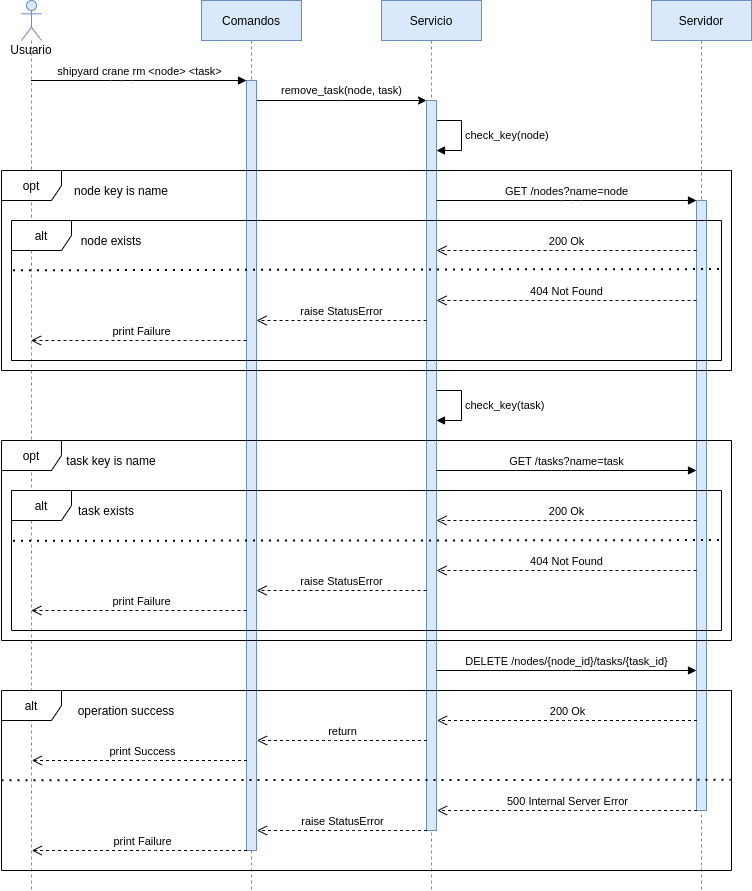
\includegraphics[width=\textwidth]{04-implementation/cli-remove-task-node.png}
              \caption{Diagrama de secuencias del comando de de eliminación de una tarea de un nodo.}
              \label{fig:04-cli_remove_task_node}
          \end{figure}

    \item \lstinline{shipyard task update <key> <values>}

          Un usuario puede actualizar una tarea usando este comando. Al igual que
          ocurría con el comando \lstinline{node update}, se pasan como argumentos
          la clave que identifica la tarea que se debe actualizar y los nuevos
          valores de los atributos en formato JSON. La clave puede ser tanto el ID
          de la tarea como su nombre. Si el usuario desea actualizar también el
          fichero \texttt{tar.gz} asociado a la tarea, debe usar la opción
          \texttt{--file} junto con la ruta del nuevo fichero.

          Tanto si la operación se realiza correctamente como si no, se imprime
          por pantalla un mensaje para informar al usuario del resultado. Cabe
          destacar que la operación del servidor a la que se llama para actualizar
          una tarea provoca la eliminación de dicha tarea de todos los nodos en
          los que se estuviera ejecutando.

    \item \lstinline{shipyard task rm <key>}

          Con este comando, el usuario puede eliminar una tarea del sistema. El
          argumento \textit{key} es la clave con la que se identifica la tarea a
          eliminar, ya sea su ID o su nombre. Al eliminar una tarea, la operación
          del servidor a la que se llama se encarga de eliminarla de todos los
          nodos en los que se estuviera ejecutando. Tanto si la operación se
          realiza correctamente como si no, se imprime por pantalla un mensaje
          para informar al usuario del resultado.

    \item \lstinline{shipyard crane deploy <node-key> <task-key>}

          Esta es, quizás, la operación más importante que se puede realizar desde
          el cliente. Permite a un usuario desplegar una tarea del sistema en un
          nodo concreto. El nodo y la tarea en cuestión se identifican por las
          claves pasadas como argumentos del comando. Estas claves pueden ser
          tanto sus IDs como sus nombres. La función del comando entonces llama a
          la función del servicio \textit{crane} encargada de enviar la petición
          HTTP al servidor para que se realice la operación. Se informa al usuario
          del resultado de la operación mediante un mensaje que se imprime en la
          terminal.

    \item \lstinline{shipyard crane rm <node-key> <task-key>}

          Al igual que el usuario puede desplegar tareas en los nodos, también
          puede retirarlas de estos usando este comando. De nuevo, el nodo y la
          tarea concretos son identificados por las claves pasadas como argumentos
          en la llamada al comando y pueden ser tanto sus IDs como sus nombres.
          Después, la función del servicio \textit{crane} se encarga de realizar
          la petición HTTP apropiada y procesar la respuesta, informando el
          comando al usuario del resultado mediante un mensaje impreso en la
          terminal. En la figura \ref{fig:04-cli_remove_task_node} se muestra en
          un diagrama de secuencias la lógica de ejecución de este comando.

    \item \lstinline{shipyard config <key> <value>}

          Este comando permite cambiar la configuración de la aplicación. Se
          debe indicar en los argumentos el parámetro a cambiar (\textit{key}) y
          el nuevo valor (\textit{value}). Se usa principalmente para
          especificar la dirección del servidor maestro.
\end{itemize}

Definir los comandos es relativamente sencillo gracias a la librería
\textit{click}. Sencillamente, definimos una función Python para cada comando y
usamos decoradores para indicar que es un comando y definir los argumentos y
opciones, de forma similar a lo que hacíamos con \textit{hug} para definir los
controladores de la API REST del servidor. En el listado de código
\ref{lst:04-cli_task_add_command} se muestra la función implementada para el
comando \texttt{shipyard task add}. Vamos a explicar qué significa cada
decorador usado:

\begin{itemize}
    \item \texttt{@task.command}: Normalmente, se usa el decorador
          \texttt{@click.command} para indicar que una función es un comando de la
          aplicación. Aquí, se usa \texttt{task} debido a que es un subcomando del
          comando base con el mismo nombre.
    \item \texttt{@click.pass\_obj}: Usado para pasar el contexto de la
          aplicación, que contiene el servicio apropiado (en este caso, el de tareas),
          a la función.
    \item \texttt{@click.option}: Son las opciones no requeridas que se pueden
          indicar en la ejecución del comando. Pueden ser de cualquier tipo y, como
          ocurre en el ejemplo mostrado, de uso múltiple.
    \item \texttt{@click.argument}: Los argumentos obligatorios del comando.
          Pueden ser de cualquier tipo.
\end{itemize}

Como se puede apreciar en el listado; el contexto, las opciones y los argumentos
son también argumentos de la función. Entrando ya en la implementación de la
operación como tal, se puede ver como se crea el objeto \texttt{Task} con los
datos dados usando un esquema definido con la librería \textit{marshmallow}.
Igual que ocurría en el servidor, usamos esta librería para facilitar el trabajo
con los recursos, haciendo muy sencillo el paso de objeto Python a diccionario y
viceversa.

\begin{lstlisting}[
    language=Python,
    caption={Comando para la creación de una nueva tarea.},
    label={lst:04-cli_task_add_command},
    showstringspaces=false
]
@task.command()
@click.pass_obj
@click.option(
    '--device', type=str, multiple=True,
    help='A device needed for the task.'
)
@click.argument('name', type=str)
@click.argument('runtime', type=int)
@click.argument('deadline', type=int)
@click.argument('period', type=int)
@click.argument('file', type=click.File('rb'))
def add(service, device, name, runtime, deadline, period, file):
    try:
        task = Task.Schema().load({
            'name': name,
            'runtime': runtime,
            'deadline': deadline,
            'period': period,
        })
        task.devices = list(d for d in device)
        new_id = service.create(task, file)
        click.echo(f'Added new task with ID {new_id}')
    except Exception as e:
        click.echo('Unable to add new task:\n' + str(e))
\end{lstlisting}

En los servicios, se hace uso de la librería \textit{requests} para realizar las
peticiones HTTP al servidor. La función del servicio de nodos encargada de su
modificación se puede ver en \ref{lst:04-cli_node_service_update}. Aquí, se
aprecia cómo se construyen estas peticiones con los disintos verbos HTTP
(\texttt{requests.get} y \texttt{requests.put}) y se gestionan las respuestas
recibidas, comprobando su código de estado para devolver un resultado o lanzar
el error correspondiente.

\begin{lstlisting}[
    language=Python,
    caption={Función del servicio de nodos para su modificación.},
    label={lst:04-cli_node_service_update},
    showstringspaces=false
]
def update(self, node_key: str, new_values: dict) -> Node:
    if not bson.ObjectId.is_valid(node_key):
        response = requests.get(
            self.base_url + '/nodes?name=' + node_key)
        if response.status_code != HTTPStatus.OK:
            raise StatusError(response.json()['error'])
        node_key = response.json()['_id']

    response = requests.put(
        self.base_url + '/nodes/' + node_key,
        json=new_values
    )
    if response.status_code == HTTPStatus.OK:
        return Node.Schema().load(response.json())
    else:
        raise StatusError(response.json()['error'])
\end{lstlisting}

\subsection{Prueba}

Para el cliente también se han implementado algunas pruebas unitarias que
validan su comportamiento, aunque solo de los comandos. Al igual que
\textit{hug}, \textit{click} proporciona mecanismos para la prueba de los
comandos implementados. En el listado \ref{lst:04-cli_task_test_setup} se
muestra el método del \textit{TestCase} de los comandos de las tareas encargado
de preparar la ejecución de las pruebas. Como se puede apreciar, se usa un
objeto \texttt{CliRunner} que simula la ejecución por consola. También se crea
una configuración de prueba. Además de esto, también es necesario maquetar el
servicio correspondiente, igual que ocurría con las pruebas de los controladores
del servidor.

\begin{lstlisting}[
    language=Python,
    caption={Función preparatoria para las pruebas de los comandos de las tareas.},
    label={lst:04-cli_task_test_setup}
]
@classmethod
def setUpClass(self):
    self.runner = CliRunner()
    self.config = Config(server_url='test', server_port='test')
\end{lstlisting}

Las funciones de prueba como tal usan este \texttt{CliRunner} para simular la
ejecución de los comandos. En el listado \ref{lst:04-cli_task_create_test} se
puede ver como se utiliza para probar el comando de creación de tareas. Con la
función \texttt{invoke}, se ejecuta el comando con distintos argumentos y
opciones y se comprueba que la salida es la correcta.

\begin{lstlisting}[
    language=Python,
    caption={Prueba del comando de creación de una nueva tarea.},
    label={lst:04-cli_task_create_test},
    showstringspaces=false
]
def test_add(self):
    with self.runner.isolated_filesystem():
        with open('test.tar.gz', 'wb') as f:
            f.write(str.encode('Test'))

        result = self.runner.invoke(
            task,
            ['add', 'Test', '1000', '1000', '1000',
                'test.tar.gz'],
            obj=self.config
        )
        self.assertIn('Added new task', result.output)

        result = self.runner.invoke(
            task,
            ['add', '--device', '/dev/null', 'Test',
                '1000', '1000', '1000', 'test.tar.gz'],
            obj=self.config
        )
        self.assertIn('Added new task', result.output)

        result = self.runner.invoke(
            task,
            ['add', 'Test1', '1000', '1000', '1000',
                'test.tar.gz'],
            obj=self.config
        )
        self.assertIn('Unable to add new task', result.output)
\end{lstlisting}

\subsection{Integración continua}

Las pruebas que se acaban de describir también se ejecutan de forma automática
cuando se realiza algún cambio en la base de código del cliente mantenida en su
repositorio de GitHub. Un flujo de trabajo casi idéntico al usado en el servidor
se encarga de lanzar estas pruebas y enviar el informe de cobertura generado a
Codecov.

No obstante, el cliente no se distribuye como una imagen Docker, como sí ocurría
con el servidor. Se ha optado mejor por publicarlo como un paquete de
PyPI\footnote{Enlace al paquete en PyPI:
    \url{https://pypi.org/project/shipyard-cli/}}, que es el repositorio de software
principal de Python, donde se encuentra la gran mayoría de paquetes y con el que
trabaja el gestor de dependencias \texttt{pip} por defecto. Para poder publicar
el paquete en esta plataforma, se añade un fichero \texttt{setup.py} a la raíz
del proyecto con los atributos del mismo (p. ej., autor, descripción,
dependencias, \dots). Luego, se define una acción en el repositorio de GitHub
que se encarga de construir el artefacto y publicarlo en PyPI cada vez que se
publique una nueva versión. Gracias a esto, el cliente se puede instalar tan
solo ejecutando \texttt{pip install shipyard-cli}.

\section{Imagen base}

\subsection{Diseño e implementación}

\subsection{Integración continua}

\section{Análisis del rendimiento}